\chapter{Form Penilaian Kenaikan Pangkat IRC}
\par
Form penilaian kenaikan pangkat IRC bertujuan untuk mengevaluasi kegiatan asisten riset IRC setiap minggunya, sehingga setiap kegiatan yang dilakukan anggota IRC akan dinilai dan dijadikan pertimbangan untuk kenaikan pangkat. penilaian ini akan didiskusikan oleh para asisten riset setiap minggunya.\\
Berikut gambaran Form Penilaian Kenaikan Pangkat IRC:
Form Penilaian Kenaikan Pangkat 1 (Mitra Tama):
\begin{figure}[H]
        \centerline{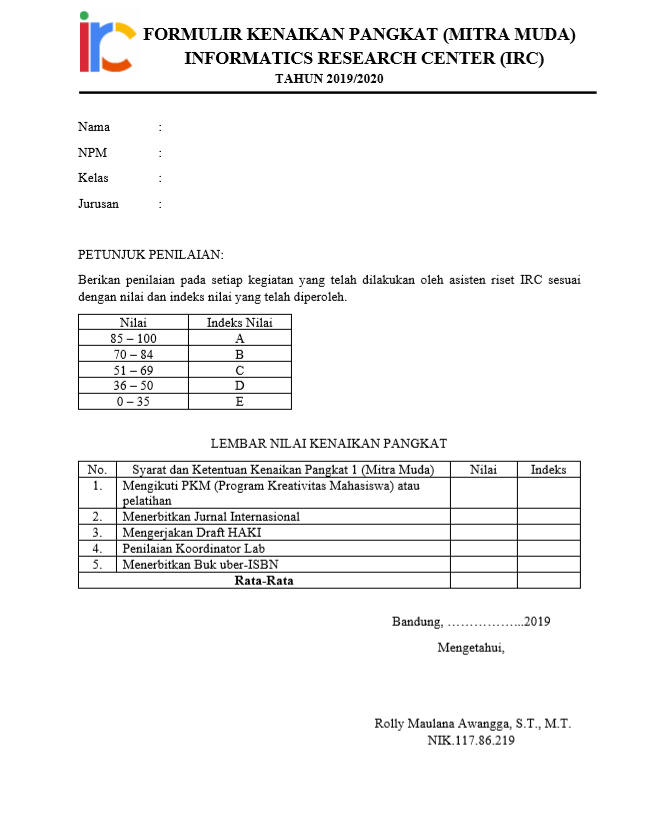
\includegraphics[scale=0.8]{figures/pangkat1}}
        \caption{Form Penilaian Kenaikan Pangkat 1}
		\label{pangkat1}
\end{figure}
Form Penilaian Kenaikan Pangkat 1 (Mitra Tama):
\begin{figure}[H]
        \centerline{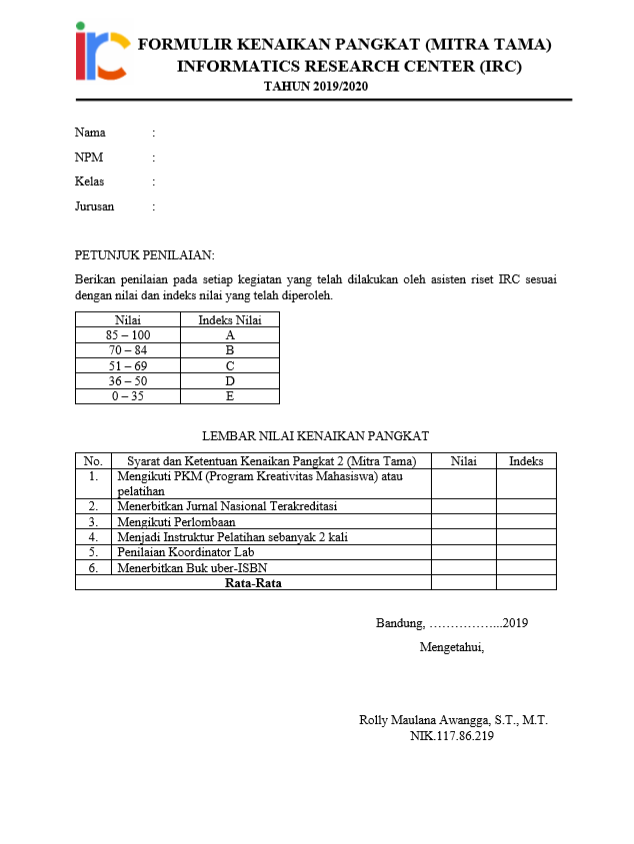
\includegraphics[scale=0.8]{figures/pangkat2}}
        \caption{Form Penilaian Kenaikan Pangkat 2}
		\label{pangkat2}
\end{figure}
Form Penilaian Kenaikan Pangkat 1 (Mitra Tama):
\begin{figure}[H]
        \centerline{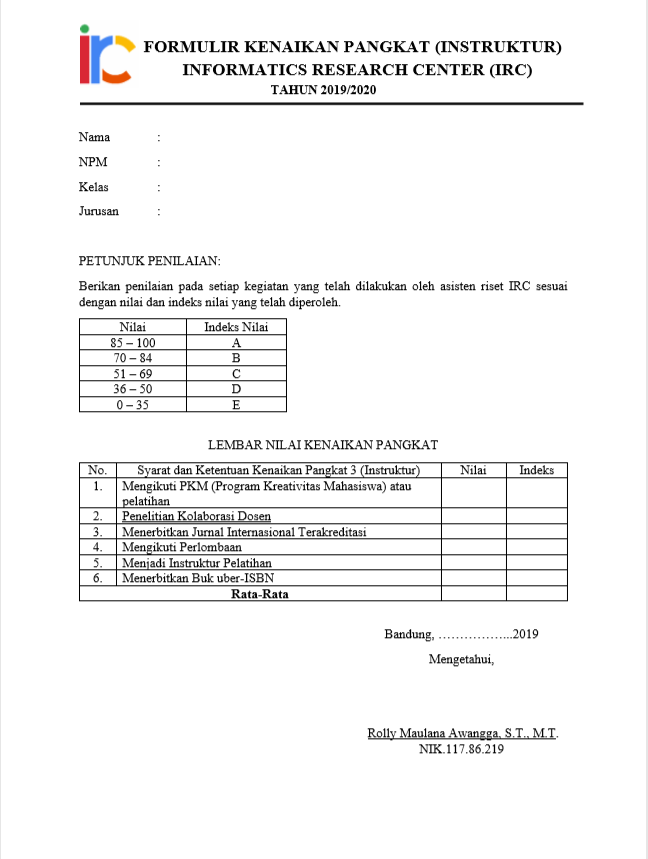
\includegraphics[scale=0.8]{figures/pangkat3}}
        \caption{Form Penilaian Kenaikan Pangkat 3}
		\label{pangkat3}
\end{figure}


